%%%%%%%%%%%%%%%%%%%%%%%%%%%%%%%%%%%%%%%%%%%%%%%%%%%%%%%%%%%%%%%%%%%%%%%%%%%%%%%%
\chapter{Концепция решения}
%%%%%%%%%%%%%%%%%%%%%%%%%%%%%%%%%%%%%%%%%%%%%%%%%%%%%%%%%%%%%%%%%%%%%%%%%%%%%%%%

В данном разделе рассмотрим технические возможности расширения поведения программы без или с минимальным вовлечением разработчика. Наибольшие технические сложности при решении поставленной задачи вызывает подстановка неявных аргументов в точку вызова определенных функций, поэтому все представленные подходы будем рассматривать с точки зрения применимости к данной проблеме. Затем приведем собственную концепцию решения, основанную на наиболее подходящем из представленных методов.

Сразу же отметим, что в рамках данной работы не рассматривались варианты, суть которых есть генерация дополнительного исходного кода перед компиляцией программы. Во-первых, автоматически генерируемый код, как правило, достаточно сложно поддерживать и фактически запрещено модифицировать. С таким положением дел можно мириться в случае, когда автоматически генерируемый код локализован, однако в случае с классами типов может понадобится модифицировать все вызовы произвольной функции (добавить неявный аргумент), которые невозможно или крайне сложно локализовать в одной небольшой части программы без потери гибкости и не нарушая основных принципов проектирования программного обеспечения. Хорошим пример здесь может служить реализация арифметических операций с помощью классов типов. Во-вторых, автоматически генерируемый код не обладает никакими привилегиями по сравнению с пользовательским кодом. Иными словами, любой сгенерированный код может быть написан пользователем самостоятельно. Здесь камнем преткновения является механизм \emph{стирания типов} (\emph{type erasure}), который имеет место быть в языках программирования семейства Java. В результате работы данного механизма во время \emph{исполнения программы} (\emph{runtime}) удаляется вся информация об \emph{обобщенных типах} (\emph{generic types}). 

Рассмотрим данную проблему более подробно. Для того, чтобы использовать функцию, описанную пусть даже в заранее известном классе типов $C$, необходимо сначала найти подходящий его экземпляр. В случае, когда точно известно для какого члена класса типов $C$ необходимо найти реализацию, задача выглядит достаточно тривиально (для ее решения можно использовать, например, программный интерфейс рефлексий (reflection api)). Пусть член класса типов неизвестен и выражается типовой переменной $T$. Тогда задача определения конкретного типа, который в действительности был использован на месте $T$, строго говоря, не может быть решена в Java подобных языках программирования. Если функция имеет хотя бы один аргумент типа $T$, то можно получить информацию о типе данного аргумента, однако здесь следует понимать, что действительный тип аргумента не имеет не имеет никакого отношения к значению $T$, выведенному на этапе компиляции. Даже если допустить, что экземпляр класса типов для типа аргумента является корректным решением, тут же возникают проблемы в случаях, когда в функции отсутствуют аргументы типа $T$ или же их более одного. Таким образом, в языках семейства Java не представляется возможным написать сколь-нибудь содержательную параметрически полиморфную функцию, которая не принимает ни одного аргумента. Здесь стоит отметить, что в языке программирования Kotlin, однако, есть механизм \emph{овеществленных типовых переменных} (\emph{reified type parameters}), который позволяет сохранить информацию о типе, который в действительности используется вместо типовой переменной. Область применения данного механизма ограничена и связана с некоторыми издержками, что не позволяет говорить о нем как о полноценном решении. Помимо этого, использование действительного типа аргументов противоречит требованию о статической типизации при разрешении классов типов.

Из-за наличия механизма стирания типов в языках программирования семейства Java также не представляется возможным реализовать необходимую функциональность в виде набора библиотечных классов и функций. На самом деле, данный механизм препятствует использованию любых инструментов, которые не работают на стадии компиляции программы, поскольку вне времени компиляции информация об обобщенных типах недоступна. 

В рамках данной работы были рассмотрены следующие инструменты модификации исходного кода программ:
\begin{itemize}
    \item Обработка аннотаций (annotation processing).
    \item Манипуляция байт-кодом программы (bytecode manipulation).
    \item Модификация компилятора языка программирования Kotlin.  
\end{itemize}

%%%%%%%%%%%%%%%%%%%%%%%%%%%%%%%%%%%%%%%%%%%%%%%%%%%%%%%%%%%%%%%%%%%%%%%%%%%%%%%%
\section{Обработка аннотаций \label{sct:concept-annotations-processing}}
%%%%%%%%%%%%%%%%%%%%%%%%%%%%%%%%%%%%%%%%%%%%%%%%%%%%%%%%%%%%%%%%%%%%%%%%%%%%%%%%

\emph{Обработка аннотаций} --- это специальный механизм Java, предназначенный для обработки аннотаций в программном коде. Для использования этого механизма необходимо реализовать и зарегистрировать собственный обработчик аннотаций. Такой обработчик будет принимать на вход абстрактное синтаксическое дерево, соответствующее аннотированному элементу программы (например, метод или тип) и модифицировать его произвольным образом. Измененное представление части программы затем передается компилятору для дальнейшей обработки в штатном режиме. 

\begin{figure}[htbp]
    \centering
    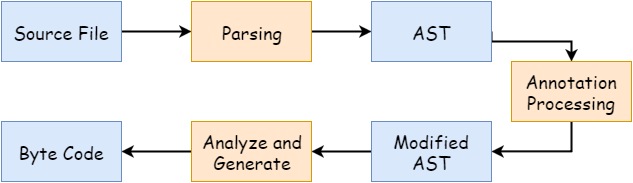
\includegraphics[width=\textwidth]{resources/05/01_annotation_processing_scheme.png}
    \caption{Схема работы механизма обработки аннотаций}
    \label{fig04:annotation-processing}
\end{figure}

Таким образом, при помощи механизма обработки аннотаций можно реализовать предварительную обработку исходного кода программы. Как и в случае автоматической генерации кода, такая обработка будет иметь место перед непосредственной компиляцией программы. По этой причине в данном подходе также не представляется возможным реализовать полноценный механизм классов типов, однако в случае обработки аннотаций по крайней мере не возникает проблемы с поддержкой стороннего исходного кода. Помимо этого, в применении к рассматриваемой задаче данная технология позволяет избежать добавления новых ключевых слов в синтаксис языка, заменив их подходящими аннотациями. Замена ключевых слов на аннотации может негативно сказаться на прозрачности и понятности нововведенных семантических конструкций, однако в то же время позволяет расширять семантику языка произвольным образом без опасения что-либо сломать.

\lstinputlisting[
    label={lst:annotation-semantic-example},
    caption={Пример введения семантики классов типов с использованием аннотаций},
    style={kotlin}
]
{resources/05/02_annotation_semantic_example}

% \begin{listing}[H]
%     \centering
%     \inputminted{kotlin}{resources/04/02_annotation_semantic_example}
%     \captionof{listing}{Пример введения семантики классов типов с использованием аннотаций}
%     \label{lst:annotation-semantic-example}
% \end{listing}

В листинге \ref{lst:annotation-semantic-example} приведен пример использования аннотаций для введения семантики классов типов в обычную программу на языке программирования Kotlin. Здесь были использованы следующие аннотации:
\begin{itemize}
    \item Аннотация \lstinline{@TypeCalss} обозначает, что объявление под ним описывает набор операций, представленных в одноименном классе типов. Область применимость данной аннотации распространяется только на объявления классов и интерфейсов.
    \item Аннотация \lstinline{@TypeClassInstance} предваряет объявление экземпляра класса типов. Два аргумента конструктора данной аннотации описывают типы класса типов и его члена соответственно. Область применимости данной аннотации ограничена объявлениями классов и объектов.  
    \item Аннотация \lstinline{@MemberOf} вводит специальное ограничение на принадлежность типовой переменной классу типов, тип которого указан в качестве единственного аргумента данной аннотации. Область применимости данной аннотации состоит только лишь из типовых переменных.
\end{itemize}

%%%%%%%%%%%%%%%%%%%%%%%%%%%%%%%%%%%%%%%%%%%%%%%%%%%%%%%%%%%%%%%%%%%%%%%%%%%%%%%%
\section{Манипуляция байт-кодом программы}
%%%%%%%%%%%%%%%%%%%%%%%%%%%%%%%%%%%%%%%%%%%%%%%%%%%%%%%%%%%%%%%%%%%%%%%%%%%%%%%%

При обычном сценарии работы программы виртуальная java-машина загружает скомпилированные классы по требованию. Технология \empph{java агентов} (\emph{java agents}) позволяет встроиться в этот процесс, определив собственный преобразователь загружаемых классов. Преобразованный произвольным образом байт-код передается затем в виртуальную java-машину и обрабатывается далее обычным образом.  

\begin{figure}[htbp]
    \centering
    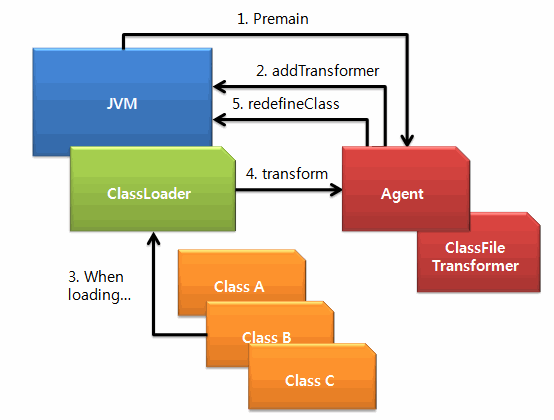
\includegraphics[width=\textwidth]{resources/05/03_bytecode_manipulation_scheme.png}
    \caption{Схема работы механизма java агентов}
    \label{fig04:java-agent-scheme}
\end{figure}

Таким образом, механизм java агентов позволяет модифицировать байт-код программы после компиляции программы, но до ее исполнения. Данный подход, как правило используется в комбинации с аннотациями, которые служат маркерами для определения мест, которые требуется модифицировать. Таким образом, семантика классов типов может быть введена как показано в листинге \ref{lst:annotation-semantic-example}. В данном подходе, конечно, недоступна информация об обобщенных типах, поэтому он также не применим к рассматриваемой задаче. 

%%%%%%%%%%%%%%%%%%%%%%%%%%%%%%%%%%%%%%%%%%%%%%%%%%%%%%%%%%%%%%%%%%%%%%%%%%%%%%%%
\section{Модификация компилятора языка программирования Kotlin}
%%%%%%%%%%%%%%%%%%%%%%%%%%%%%%%%%%%%%%%%%%%%%%%%%%%%%%%%%%%%%%%%%%%%%%%%%%%%%%%%

Исходный код компилятора Kotlin насчитывает более двадцати тысяч файлов. Таким образом, модификация компилятора Kotlin является весьма трудоемкой задачей. Особенно данный факт усугубляется отсутствием качественной документации, описывающей внутреннее устройство компилятора. Кроме того, стоит отметить, что при использование данного подхода к рассматриваемой задаче реализации механизма классовых типов, добавляются задачи корректировки анализатора языка таким образом, чтобы пользователю предоставлялась правильная информация об ошибках, а также модификаций синтаксической структуры языка в случае необходимости добавления новых языковых конструкций. Конечно, данный подход дает наибольшую гибкость и, как следствие, наибольшие гарантии разрешимости задачи. Стоит, однако, понимать, что исходный код компилятора может быть спроектирован таким образом, что добавление необходимой функциональности будет практически равносильно написанию собственного компилятора.

%%%%%%%%%%%%%%%%%%%%%%%%%%%%%%%%%%%%%%%%%%%%%%%%%%%%%%%%%%%%%%%%%%%%%%%%%%%%%%%%
\section{Выводы}
%%%%%%%%%%%%%%%%%%%%%%%%%%%%%%%%%%%%%%%%%%%%%%%%%%%%%%%%%%%%%%%%%%%%%%%%%%%%%%%%

Все методы, рассмотренные выше, кроме подхода, подразумевающего модификацию компилятора, не позволяют реализовать механизм классов типов в требуемом объеме и в соответствии с выдвинутыми требованиями. Таким образом, здесь мы фактически вынуждены использовать именно этот подход. Для упрощения задачи не будем рассматривать вариант модификации синтаксиса языка путем добавления новых ключевых слов. Во-первых, как видно из листинга \ref{lst:annotation-semantic-example}, мощности аннотаций вполне достаточно для того, чтобы ввести необходимую семантику. Во-вторых, отсутствует общепринятая грамматика для описания синтаксиса Kotlin. В частности, синтаксис, используемый внутри компилятора несколько отличается от доступного пользователям. Стоит отметить, что ограничение на принадлежность типовой переменной классу типов, как оно представлено в примере \ref{lst:annotation-semantic-example}, не позволяет выразить подобное ограничение для более чем одной типовой переменной. Есть два варианта решения данной проблемы:
\begin{enumerate}
    \item \label{it04:solution-1} В аннотацию \lstinline{@MemberOf} добавляется дополнительный аргумент, выражающий позицию типовой переменной в шаблоне класса типов. 
    \item \label{it04:solution-2} Ограничение на принадлежность типовой переменной $T$ классу типов $C$ может быть выражено следующим образом: существует тип $I$ такой, что $I$ является наследником типа $C$ с параметром $T$.
\end{enumerate}
В данном случае вариант \ref{it04:solution-2} выглядит лучше, по следующим причинам:
\begin{itemize}
    \item Компилятор автоматически проверит ограничения на типовые переменные в случае, если таковые имеются.
    \item При необходимости в будущем аннотацию \lstinline{@MemberOf} можно будет убрать.
\end{itemize}
Кроме того, аннотация \lstinline{@TypeClassInstance} является избыточной, поскольку информацию, указанную в ее аргументах можно вычислить из списка супер типов класса. Целесообразным представляется отказаться от использования данной аннотации. В противном случае необходимо реализовать механизм проверки аргументов аннотации на соответствии списку супер типов, что может привести к не очевидным с точки зрения пользователя ошибкам. Таким образом, пример \ref{lst:annotation-semantic-example} можно переписать как показано в листинге \ref{lst:concept-example}. В данном примере для удобства используется уже единственная аннотация \lstinline{@TypeClass} с семантикой, аналогичной семантике аннотаций \lstinline{@TypeClass} и \lstinline{@MemberOf} в случаях объявления класса типов и наложения ограничения на принадлежность типовой переменной некоторому классу типов. 

\lstinputlisting[
    label={lst:concept-example},
    caption={Пример введения семантики классов типов с использованием аннотаций},
    style={kotlin}
]
{resources/05/04_concept_example}

% \begin{listing}[H]
%     \centering
%     \inputminted{kotlin}{resources/05/04_concept_example}
%     \captionof{listing}{Пример введения семантики классов типов с использованием аннотаций}
%     \label{lst:concept-example}
% \end{listing}